\documentclass{article}

% UniReps 2026, full paper track (archival): at most 9 pages of main text.
\usepackage[dblblindworkshop]{neurips_2026}
\workshoptitle{UniReps}
\makeatletter
\renewcommand{\@noticestring}{Submitted to the UniReps Workshop. Do not distribute.}
\makeatother

\usepackage[utf8]{inputenc}
\usepackage[T1]{fontenc}
\usepackage{hyperref}
\usepackage{url}
\usepackage{booktabs}
\usepackage{array}
\usepackage{amsfonts,amsmath,amssymb,amsthm}
\usepackage{nicefrac}
\usepackage{microtype}
\usepackage{xcolor}
\usepackage{graphicx}
\usepackage{caption}
\graphicspath{{../figures/}}

\newtheorem{proposition}{Proposition}
\newtheorem{corollary}{Corollary}
\newcommand{\dprime}{$d'$}
\newcommand{\gpuhours}{51}

\title{A Shared Readout Bottleneck across Language Models\\and Human Working Memory}

\author{%
  Anonymous Author(s) \\
  Affiliation \\
  Address \\
  \texttt{email} \\
}

\begin{document}

\maketitle

\begin{abstract}
Large language models (LLMs) reproduce a human working-memory signature on the N-back task: performance declines as memory load N increases, and errors concentrate on lures, items that repeat the current stimulus at a neighboring but incorrect serial position. Does a shared behavioral signature reflect a shared mechanism? On a \emph{precision} account, softmax attention cannot concentrate weight on that item, so adjacent items are retrieved instead. On an \emph{interference} account, as proposed for human working memory, attention selects the correct item, but the content of competing items corrupts the decision. We dissociate these accounts in 15 pretrained LLMs from three families (70 million to 14 billion parameters) and in minimal transformers trained from scratch. Every family gives the same answer. The attention heads that carry the task attend to the target on most missed matches. Linear probes decode near-perfectly whether a matching letter occurred at the target or at a lure position, even on trials where the model false-alarms to the lure: the information is decodable but unused. Sharpening attention yields negligible gains, whereas suppressing the letter identity of non-target items improves sensitivity (\dprime{}) in 42 of 43 model-by-load conditions. With scale, the task becomes spread over more heads, yet the benefit of removing interference grows. A single-layer transformer is limited by precision, but a second layer removes this limit. Distinct networks thus converge, with each other and with humans, on a common bottleneck: not locating items but reading them out under interference.
\end{abstract}

\section{Introduction}
\label{sec:intro}

Working memory, the ability to hold a few pieces of information in mind and use them, is famously limited in humans \citep{cowan2001magical,ma2014changing}. A standard probe is the N-back task \citep{kirchner1958age}: people watch a stream of letters and, for each one, say whether it matches the letter N positions earlier. Performance falls steeply as N grows, and the errors are telling. People most often false-alarm on \emph{lures}, letters that repeat the current one at a nearby but wrong distance, such as N$-$1 or N$+$1 back \citep{kane2007nback}. A lure error shows that the letter was remembered but its position was confused, and such errors are usually explained as a failure to select the target against competing items \citep{engle2002executive,oberauer2012interference,szmalec2011interference}.

Large language models (LLMs) show the same signature \citep{gong2024chatgpt,hu2025nback,xiong2026superposition}. This is surprising. An LLM does not need to hold earlier items in a limited store: the whole sequence stays in its input, and at every step it can look back at any earlier item through \emph{attention} \citep{vaswani2017attention}. Roughly, the current position gives every earlier position a score, the scores are turned into weights that sum to one, and the model takes the weighted average of what the earlier positions contain. Because nothing is forgotten, the limit must arise when the model retrieves an earlier item and uses it to decide.

The shared signature raises a question central to comparing neural systems: do networks that behave alike compute alike? Similar errors can arise from different mechanisms, and representations that look alike to a decoder need not play the same role in behavior. N-back offers a sharp test: two accounts that predict the same lure errors make opposite predictions about the model's internals, which can be checked across model families and sizes and compared with accounts of human working memory.

Where could this process fail? Two accounts have been proposed (Fig.~\ref{fig:overview}b). On the first, the \emph{precision} account, the model fails to locate the target. Attention weights are computed by a softmax, a form of divisive normalization \citep{carandini2012normalization}: each position's weight is its own (exponentiated) score divided by the sum over all positions, so positions compete for weight. The target's immediate neighbors lie only one position away from it (N$\pm$1 back), so if the model cannot tell adjacent positions apart sharply, they receive scores almost as high as the target's, and part of the weight spills onto them. A lure error then occurs because attention lands partly on the lure and the model reads its letter. This account was proposed for small transformers trained on N-back \citep{gong2024selfattention} and is supported by analyses of softmax \citep{velickovic2025softmax}. On the second, the \emph{interference} account, the model locates the target but fails to read it out correctly. Attention lands on the target, but inside the model the target's content is mixed with the content of other recent items, and the mixture corrupts the decision. \citet{xiong2026superposition} found evidence for this account: the models' errors are biased toward recent items, item representations overlap inside the models, and suppressing letter-identity directions can improve performance. But the precision account also predicts errors biased toward neighbors, and attention averaged over trials, which peaks at the target but keeps weight on its neighbors, does not show where attention goes when the model errs. The two accounts have not been tested against each other.

The two accounts make different predictions. If the precision account is right, attention should be off target when the model errs, and sharpening attention should help. If the interference account is right, attention should be on target even on errors, the information needed for the correct answer should be present in the model, and removing the competing content, not sharpening attention, should help.

We test these predictions in 15 pretrained LLMs and in small transformers trained from scratch, where the precision account can be analyzed exactly. The answer is consistent across models: LLMs find the item but misread it. The attention heads that carry the task attend to the target on most errors, and a simple classifier reads from the model's own activations whether a repeated letter sat at the target or at a lure position, even on the trials where the model falls for the lure (Section~\ref{sec:locate}). Causally, erasing the content of competing items improves performance far more than sharpening attention does (Section~\ref{sec:causal}; Fig.~\ref{fig:overview}c). The same dissociation holds in every family and across a 200-fold range of size; what changes with scale is the circuit, which becomes more distributed, not the bottleneck. The precision account is not wrong but narrow: it holds in a transformer with a single attention layer, and a second layer removes it (Section~\ref{sec:theory}).

\begin{figure}[t]
  \centering
  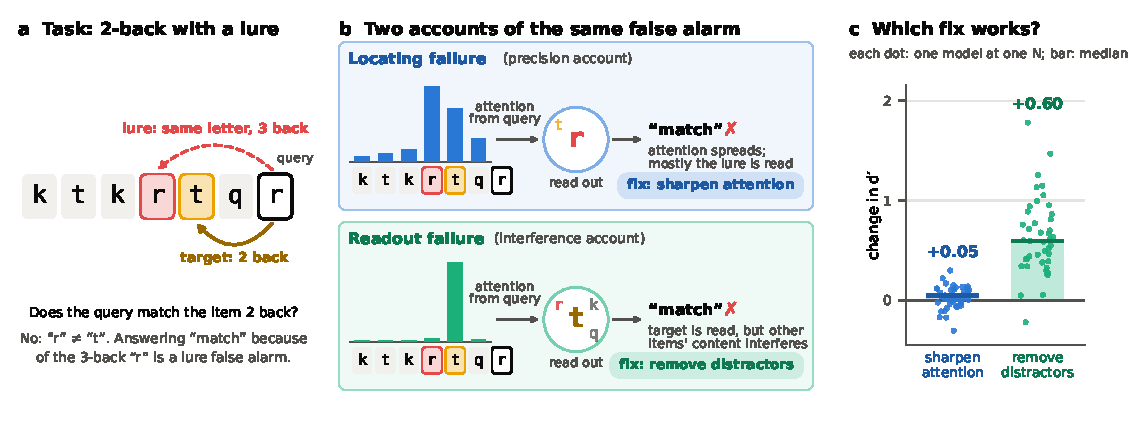
\includegraphics[width=\textwidth]{fig1_overview.pdf}
  \caption{\textbf{Two accounts of the same error.} (a) In 2-back, the query ``r'' must be compared with the item two back (``t''). The ``r'' three back is a lure: answering ``match'' because of it is a lure false alarm. (b) Attention lands on the lure and reads its letter (precision account; fix: sharpen attention), or lands on the target while other items' letters leak into the decision (interference account; fix: remove the distractors' content). (c) Across 15 LLMs and N = 2--4 (dots: one model at one N; bars: medians), sharpening the task's heads barely changes sensitivity \dprime{}, whereas removing the letter identity of non-target items raises it in 42 of 43 cases (Section~\ref{sec:causal}).}
  \label{fig:overview}
\end{figure}

\section{Task, models and measures}
\label{sec:setup}

\textbf{The N-back task.} Each sequence has 24 letters drawn from 20 consonants. For each letter, the \emph{query}, the correct answer is ``match'' if it equals the letter N positions back, the \emph{target}, and ``no match'' otherwise. Each test sequence contains four lures: letters that repeat the query at N$\pm$1 or another non-target distance without creating a match.

\textbf{Presenting the task to LLMs.} A one-sentence instruction and three solved example sequences are followed by the test sequence, one item per line, each line holding a letter and its answer (``\texttt{k -}'' for no match, ``\texttt{t m}'' for match). The answers to earlier items are shown correctly, so the model never builds on its own mistakes. We take the model's decision at each letter to be its preference for ``\texttt{m}'' over ``\texttt{-}'' (the difference of their log-probabilities). A threshold set on 200 separate calibration sequences turns this preference into a yes/no answer, and all results use 1,000 further test sequences per model and N.

\textbf{Measuring performance.} As in human studies, we report sensitivity \dprime{} from signal detection theory \citep{hautus1995corrections}: how far apart the model's responses to matches and non-matches lie, in units of their spread. \dprime{} is 0 at chance and, unlike accuracy, is not inflated by a bias toward answering ``no match''. We also report hit rates and false-alarm rates, separately for lures and for other non-matches.

\textbf{Models.} We test 15 pretrained models from three families: Pythia, seven sizes from 70M to 6.9B parameters \citep{biderman2023pythia}; GPT-2, four sizes from 124M to 1.5B \citep{radford2019gpt2}; and Qwen2.5, four sizes from 0.5B to 14B \citep{qwen2025qwen25}. Section~\ref{sec:theory} also uses small transformers trained from scratch on N-back (Appendix~\ref{app:methods}).

\textbf{Two terms from inside a transformer.} Each layer contains several \emph{attention heads}; each head computes its own attention pattern and writes its own output, and a few heads often do most of the work for a given task \citep{elhage2021framework,olsson2022induction,wu2024retrieval}. The model also keeps, for each position, a running vector that every layer reads from and adds its output to. This \emph{residual stream} is the model's working representation of that position. To find the heads that carry N-back, we use activation patching \citep{zhang2024patching}. We run the model on two sequences that differ only in the target letter, so that the correct answer flips, and copy the output of a single head from the first run into the second. A head whose output alone moves the answer a long way back toward the first run's answer is important for the task. One head usually dominates and is the same across N; at N = 2 it alone recovers 16--73\% of the difference between the two runs, depending on the model.

\section{LLMs show a human-like load effect and lure errors}
\label{sec:behaviour}

As in earlier studies \citep{gong2024chatgpt,hu2025nback,xiong2026superposition}, all 15 models get worse as N grows (Fig.~\ref{fig:behaviour}a--c; Table~\ref{tab:l2}). Median \dprime{} falls from 2.57 at N = 1 (range 1.25--4.28) to 0.91 at N = 4 and 0.52 at N = 6. Scale helps when the task is easy but much less when it is hard: the largest model, Qwen2.5-14B, reaches 4.28 at N = 1 but only 1.15 at N = 6. As in humans and in \citet{xiong2026superposition}, errors concentrate on lures (Fig.~\ref{fig:behaviour}d). At N = 2, models answer ``match'' to a median 79\% of lures at N$\pm$1, against 4\% of other non-matches.

Two checks rule out trivial explanations. Weaker models can drift to an easier task \citep{hu2025nback}, but the $k$-back rule that best fits the answers differs from N in only 14 of 90 cases, all at N$\,\ge\,$4 in small models. And a chat format, one letter per turn as in \citet{gong2024chatgpt}, gives the same decline in Qwen2.5-Instruct 0.5B--7B (\dprime{} 1.8--2.0 at N = 1, 0.4--0.7 at N = 6).

The lure errors pose our question. When a model false-alarms on a lure, did it look in the wrong place, or did it look in the right place and misread what it found?

\begin{figure}[t]
  \centering
  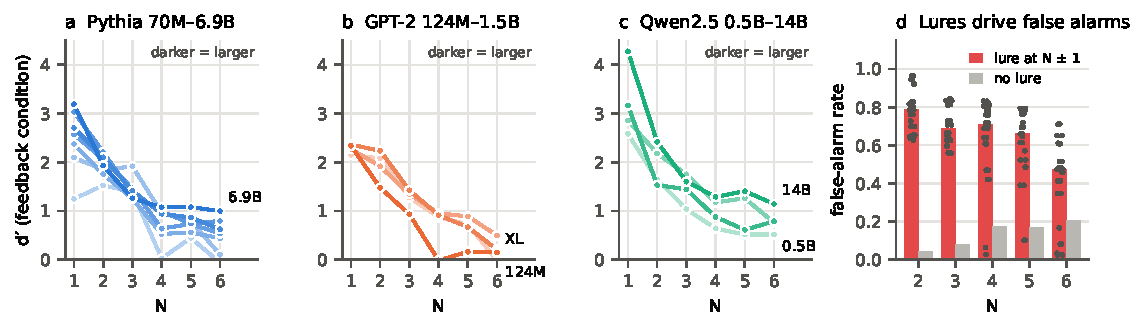
\includegraphics[width=0.88\textwidth]{fig3_llm_behaviour.pdf}
  \caption{\textbf{LLMs decline with N and fall for lures.} (a--c) Sensitivity \dprime{} against N for three model families; darker lines are larger models. (d) False-alarm rates on lures at N$\pm$1 (red; dots are models) and on other non-matches (gray), medians over 15 models.}
  \label{fig:behaviour}
\end{figure}

\section{LLMs find the target but misread it}
\label{sec:locate}

\textbf{Attention lands on the target, even on errors.} We first ask where the task's heads look. For each query, we measure how much attention the five most important heads send from the query letter to the target's line (its letter, answer and line break) and to the lines just before and after it. We say the heads \emph{locate} the target when its line receives at least as much attention as either neighbor.

On correctly answered matches, the heads locate the target on a median 88--91\% of trials (14 models; GPT-2 Large is excluded because its top heads attend to none of the three lines). On correctly answered non-matches, they do so on only about 25\%. This contrast shows how the heads work: they search by content, attending to where the query's letter appeared, which on a match trial is the target.

The critical trials are the misses, matches that the model calls ``no match''. If misses came from imprecise attention, attention should be off target on them. It rarely is: the heads look elsewhere on only 16\%, 7\% and 8\% of misses at N = 2, 3 and 4 (Fig.~\ref{fig:locate}a). Where, then, does the answer go wrong? A classifier trained on correct trials to read the answer from the heads' outputs gives a split. On 41--57\% of misses, the heads' outputs already pointed to the wrong answer although their attention was on the target: what they carried was contaminated. On 27--43\%, the outputs pointed to the right answer, which was lost in later layers. In both cases the target had been found.

Lure false alarms look different at first sight. On 91--96\% of them a neighboring line, typically the lure's, receives more attention than the target. But this is what a head that searches by content should do: on a lure trial the query's letter sits at the lure, so that is where the head looks. Finding the lure is not the mistake. The mistake is to treat it as a match, and avoiding it requires knowing that the matching letter sat at N$\pm$1 rather than at N. Does the model know this?

\textbf{The model knows where the match was.} Matches and lures both contain the query's letter; only its position differs. We trained a linear probe, a logistic-regression classifier, to tell matches from lures using the residual stream at the query, separately at nine depths and with training and test sequences kept apart. If such a probe succeeds, the information is present in a form that a single linear unit downstream could read. We score both the probe and the model's own decision by the area under the ROC curve (AUC): the probability that a randomly chosen match scores higher than a randomly chosen lure, which is 0.5 at chance and 1 when the two are perfectly separated.

The gap is striking (Fig.~\ref{fig:locate}b,c). The model's own decision separates matches from lures barely above chance (median AUC 0.63 at N = 2, 0.58 at N = 3). A probe reading the same model's activations separates them almost perfectly (median 1.00 and 0.98 at the best depth). Because the input embeddings are at chance, this is information the model computes, not information it is given. Most importantly, it is present on the trials the model gets wrong: on the model's own lure false alarms, the probe still classifies a median 95\% (N = 2) and 86\% (N = 3) as lures. In the largest model, Qwen2.5-14B, the model's own AUC is 0.81 and 0.64, the probe's 1.00 and 0.997, and the probe recognizes 99.8\% and 95\% of the model's lure false alarms as lures. The information peaks in middle layers and fades toward the output, as relative-position information does in \citet{xiong2026superposition}.

The models therefore locate the target and compute where the matching letter was, but their decision does not use what they computed. The bottleneck lies after locating, in readout.

\begin{figure}[t]
  \centering
  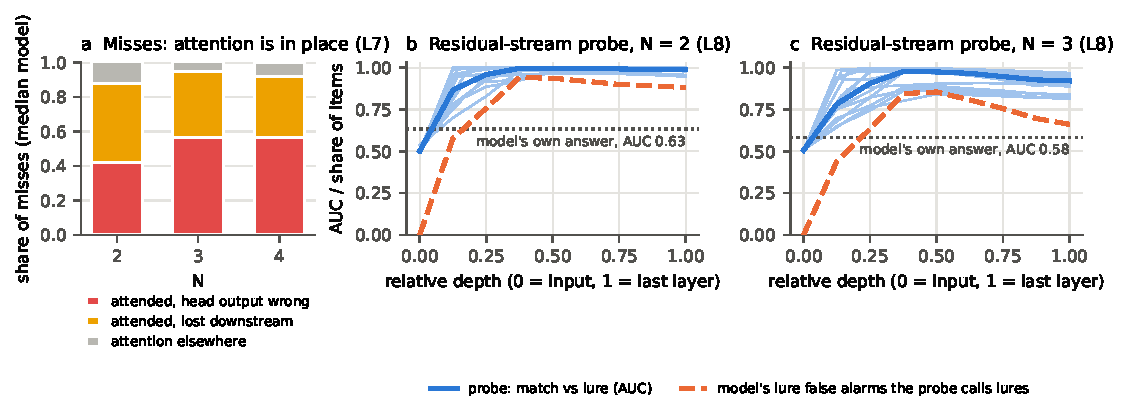
\includegraphics[width=\textwidth]{fig4_locate_vs_readout.pdf}
  \caption{\textbf{LLMs find the target but misread it.} (a) Misses, split by whether the top heads attended to the target and, if so, whether their output already pointed to the wrong answer (median over 14 models). Attention is off target on few misses. (b, c) A linear probe on the residual stream separates matches from lures (blue; thin lines are individual models, thick line the median) far better than the model's own decision (dotted), and classifies most of the model's own lure false alarms as lures (orange). Depth is scaled from the input (0) to the last layer (1).}
  \label{fig:locate}
\end{figure}

\section{Removing interference helps; sharpening attention does not}
\label{sec:causal}

The evidence so far is correlational. Heads might attend to the target yet pass on a blurred copy of it that sharper attention would clean up. We therefore intervene on the models. If the interference account is right, removing the content of competing items should help more than sharpening attention. We apply each intervention to all 15 models at N = 2--4 on the same sequences, recalibrating the decision threshold each time (Fig.~\ref{fig:causal}a; Table~\ref{tab:b1}). Each intervention is compared with the unmodified model by a paired bootstrap over sequences (95\% intervals, 2,000 resamples). Two cases whose baseline \dprime{} is below 0.3 are excluded, leaving 43 model-by-N cells.

\textbf{The identified heads are necessary.} Replacing the outputs of the ten most important heads with their average over calibration items, which removes the trial-specific information they carry, lowers \dprime{} in 42 of 43 cells (median $-0.93$). Ten random heads from the same layers do nothing (median $+0.00$).

\textbf{Sharper attention barely helps.} Dividing the attention scores of the top three heads by a temperature $\tau<1$ before the softmax concentrates their attention. This changes \dprime{} by a median $+0.05$ at $\tau=0.67$ and $+0.03$ at $\tau=0.8$ (range $-0.30$ to $+0.30$). The gain is consistent (Wilcoxon $p=0.04$ and $0.001$) but small. Flattening the same heads ($\tau=2$) costs a median 0.32, and when we change the temperature of every head in the model, mild \emph{flattening} ($\tau=1.25$) is best in 19 of the 30 cells tested. The heads already sit near their best sharpness.

\textbf{Removing distractor content helps a lot.} We first find the directions in the residual stream that encode letter identity: the 19-dimensional subspace spanned by the average activations of the 20 letters (after subtracting their mean), estimated on calibration sequences. Then, for each query, we remove half of each earlier item's component in this subspace, at every layer and over the item's whole line, sparing only the target. This leaves the target and the positions of all items intact but blurs which letter each distractor was. It raises \dprime{} in 42 of 43 cells (median $+0.60$, up to $+1.78$), including at N = 4 (median $+0.44$). It does so the way the interference account predicts: false alarms fall from about 0.2--0.3 to about 0.1 while hits hold. Two controls show that the effect is specific. Removing a random subspace of the same size does nothing (median $-0.03$), and removing the target's letter instead destroys performance (median $-1.54$). Complete removal also helps (median $+0.46$) but over-suppresses in Qwen2.5-7B. Because this intervention needs to know which item is the target, it is a causal test of interference, not a usable method. Replicating the single-direction removal of \citet{xiong2026superposition} at answer positions, with its configuration chosen on calibration sequences, gives a median $+0.11$ (28 cells; $+0.12$ when chosen on the test trials, as in the original study), about a fifth as much. Their gains were largest in the weakest models; ours grow with model size (below). Distractor suppression and head ablation both differ from zero with Wilcoxon $p<10^{-8}$.

\textbf{Why sharpening can do so little.} A simple model of the readout explains this ordering. The quantity the model decides on contains the signal (does the query match the target?) plus the letter content of other items, written in by many heads in many layers. Sharpening one head removes only the distractor content that this head contributes, which is small when the head already attends mostly to the target. Removing distractor content acts wherever that content was written.

\begin{proposition}[sharpening versus removing interference]\label{prop:interference}
Let the decision variable be $r=w^\top h$ with $h=\gamma\,y\,e+\sum_{j\in D}B_j g_j+z$, where $y=\pm1$ marks match and non-match, $\gamma e$ is the signal, $g_j\in\mathbb{R}^d$ is the letter content of distractor item $j\in D$, which lies in a $q$-dimensional subspace, $B_j$ are fixed linear maps that write it into $h$, and $z$ is noise independent of the letters. Distractor content may depend on $y$ (lures occur on non-match trials): let $b_y=\mathbb{E}[w^\top\sum_jB_jg_j\mid y]$, $\beta=b_{+}-b_{-}$, and let $\sigma_D^2$ and $\sigma_z^2$ be the within-class variances of the distractor and noise terms of $r$. Then $d'=(2\gamma\,w^\top e+\beta)/\sqrt{\sigma_D^2+\sigma_z^2}$.
\begin{enumerate}\setlength{\itemsep}{1pt}\setlength{\topsep}{2pt}
  \item[(a)] Removing a fraction $\alpha$ of every distractor's letter content ($g_j\to(1-\alpha)g_j$) gives $d'(\alpha)=(2\gamma\,w^\top e+(1-\alpha)\beta)/\sqrt{(1-\alpha)^2\sigma_D^2+\sigma_z^2}$, which increases with $\alpha$ when $\beta\le0$, that is, when distractors push non-match trials toward ``match'', as lures do.
  \item[(b)] Removing a uniformly random $q$-dimensional subspace instead removes, in expectation, a fraction $q/d$ of each distractor's content (in squared norm).
  \item[(c)] If a head with value vectors $v_j$ and output $W_O\sum_j a_j v_j$ reaches $h$ directly and puts attention weight at least $1-\epsilon$ on the target line, it contributes at most $\epsilon\max_j|w^\top W_O v_j|$ of distractor content to $r$; this bounds what re-weighting its attention can remove.
\end{enumerate}
\end{proposition}

The proposition's predictions match the data: suppression lowers false alarms while sparing hits, by removing both the lure bias $\beta$ and the variance $\sigma_D^2$; a random subspace removes almost nothing ($q/d\le19/512$); and sharpening is bounded by the small off-target share of a few heads. The model does not explain why half-strength removal beats full removal; complete removal may push activations outside their usual range. Proofs are in Appendix~\ref{app:theory}.

\textbf{What scale changes, and what it does not.} Comparing models of different sizes asks which parts of the mechanism are shared. The two interventions part ways as models grow (Fig.~\ref{fig:causal}b). Ablating the identified heads costs less in larger models (Spearman $\rho=0.74$ between size and each model's median change, $p=0.002$, 15 models), from about $-1.6$ in the smallest Pythia models to $-0.21$ in Qwen2.5-14B: the solution becomes more distributed across heads. Yet removing distractor content helps more in larger models ($\rho=0.57$, $p=0.03$). Qwen2.5-14B shows this most clearly. Half-strength suppression raises its \dprime{} from 2.42 to 2.88, from 1.60 to 3.38 and from 1.29 to 2.05 at N = 2, 3 and 4, with every bootstrap interval at least 0.40 above zero, while a random subspace changes it by $-0.10$, $-0.05$ and $+0.18$. With distractor content removed, the model does better at 3-back than it does unaided at 2-back. Across a 200-fold range of size, the circuit that implements the task changes, but the bottleneck it runs into does not.

\begin{figure}[t]
  \centering
  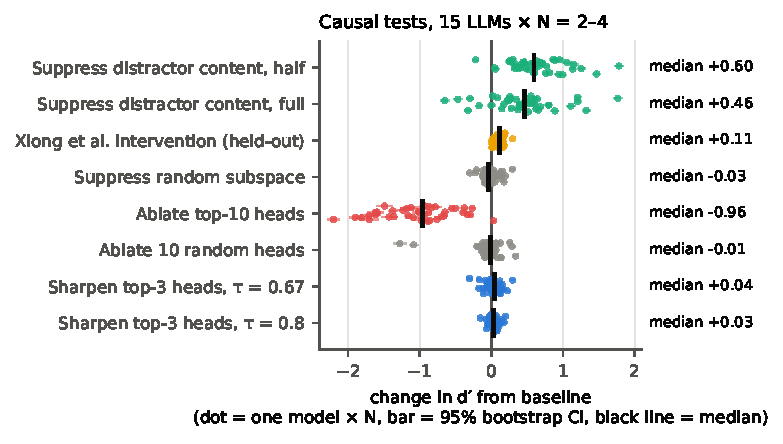
\includegraphics[width=\textwidth]{fig5_causal_tests.pdf}
  \caption{\textbf{Removing interference helps; sharpening attention does not.} (a) Change in \dprime{} from the unmodified model under each intervention. Each dot is one model at one N with its 95\% bootstrap interval; black lines are medians. (b) Each model's median change over N = 2--4 against its size, for removing distractor content (half strength) and ablating the top ten heads; lines are least-squares fits against log size.}
  \label{fig:causal}
\end{figure}

\section{Where attention precision does bind}
\label{sec:theory}

\begin{figure}[t]
  \centering
  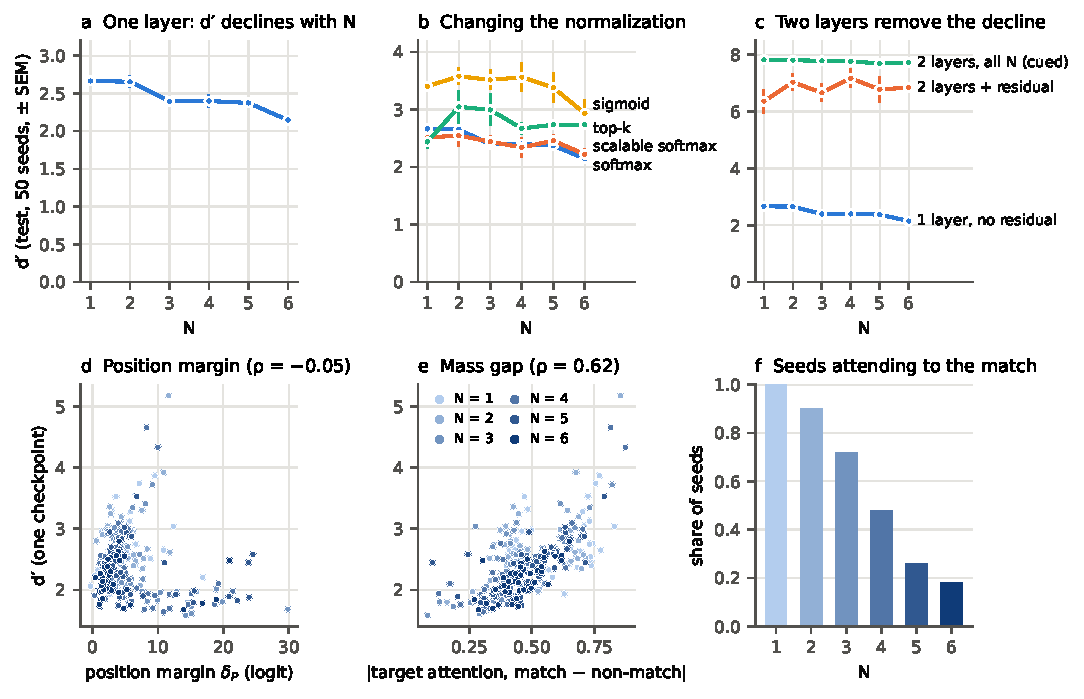
\includegraphics[width=\textwidth]{fig2_minimal_models.pdf}
  \caption{\textbf{Where attention precision binds: minimal transformers trained from scratch.} (a) A one-layer model without residual stream declines with N (50 seeds, $\pm$SEM). (b) Sigmoid and top-$k$ attention flatten the decline; scalable softmax does not. (c) Two layers with a residual stream remove it, both for one model per N and for one cued model trained on all N. (d, e) Across 300 one-layer models (50 seeds $\times$ N = 1--6; darker = larger N), \dprime{} is unrelated to the position margin $\delta_P$ but tracks how much attention to the target differs between match and non-match trials. (f) Share of models that attend more to the target on match trials.}
  \label{fig:minimal}
\end{figure}


If LLMs locate the target, why has the precision account seemed compelling? It was proposed for a minimal transformer: a single attention layer with no residual stream and no further processing, trained on N-back \citep{gong2024selfattention}. Such a model does decline with N (\dprime{} from 2.67 to 2.15 over N = 1--6; Fig.~\ref{fig:minimal}a). We trained one such model for each N from 50 random seeds, 300 models in all, and refer to them as the main models. Here we analyze it exactly, ask what limits it, and ask whether the limit survives a second layer.

\textbf{The minimal model.} For a query at position $i$, the model attends with weights $a_{ij}$ to every position $j$ and outputs $o_i=\sum_j a_{ij}v_j$, where $v_j$ is the value vector of item $j$; the decision is a linear function of $o_i$. Attention scores have a content term and a position term, $s_{ij}=c(x_i,x_j)+p(i-j)$, where $x_j$ is the letter at $j$. Let $t=i-N$ be the target, $u_j=w^\top v_j$ the amount item $j$ adds to the decision, and $r_i=\sum_j a_{ij}u_j$ the decision variable. Without a residual stream, $u_j=u(x_j,j)$ depends only on the letter and position of item $j$. Our sequences treat all letters alike, so every single position has the same letter distribution on match and non-match trials; only the joint distribution of letters differs.

\textbf{A one-layer model can detect a match only through where it attends.} The output is a weighted average of letter vectors, and a weighted average with fixed weights cannot tell whether two letters are equal. The comparison must therefore happen in the attention weights themselves.

\begin{proposition}[the readout is a test of attention mass]\label{prop:mass}
In this model the decision is linear in $\sum_j a_{ij} v_j$, and for fixed weights $a_{ij}$ no linear function of a convex combination of letter embeddings can test whether two letters are equal. The difference in mean readout between match and non-match trials must therefore be carried by how the attention distribution differs between them.
\end{proposition}

\begin{corollary}[precise location without content carries no signal]\label{cor:fixed}
For any fixed weight vector $\bar a$ and $u_{\max}=\max_{x,j}|u(x,j)|$,
\[
\bigl|\mathbb{E}[r_i\mid\text{match}]-\mathbb{E}[r_i\mid\text{non-match}]\bigr|\;\le\;u_{\max}\bigl(\mathbb{E}_{\text{match}}\|a_i-\bar a\|_1+\mathbb{E}_{\text{non-match}}\|a_i-\bar a\|_1\bigr).
\]
In particular, any attention pattern that does not depend on content, including one that splits all weight between $i$ and $i-N$, gives the same mean readout on match and non-match trials, however precisely it locates the target.
\end{corollary}

Both statements hold in trained models. We took the 300 main models, together with 420 variants that differ in width, amount of training data or weight decay (720 one-layer models in all), and replaced their attention by a fixed mix of positions $i$ and $i-N$, so that both letters reach the output: \dprime{} stays within $\pm0.07$ of zero at every N. Removing the content term from the attention scores gives the same result ($|d'|\le0.04$). Precise location is useless unless attention responds to content. What does predict performance is how much attention to the target \emph{changes} between match and non-match trials: across the 300 main models, the size of this change correlates with \dprime{} at Spearman $\rho=0.62$ (Fig.~\ref{fig:minimal}e). Its sign changes with N. At N = 1 every model attends more to the target when it matches; at N = 4 only 48\% do and at N = 6 only 18\%, while the rest attend \emph{away} from a matching letter (panel f). Both strategies test where the attention mass goes, and Corollary~\ref{cor:fixed} constrains them alike.

\textbf{Softmax normalization matters, but not through precision.} The precision account rests on a property of softmax: competing positions dilute the target's weight.

\begin{proposition}[softmax dispersion]\label{prop:dispersion}
If each of the $K$ other positions has a score at least $\Delta$ below the target's, the target receives weight at least $1/(1+Ke^{-\Delta})$, and this guarantees weight $1-\epsilon$ for every such configuration if and only if $\Delta\ge\log(K(1-\epsilon)/\epsilon)$. Two positions with the same letter are separated only by the position term: an item at distance $N\pm1$ receives $e^{-\delta_P}$ times the weight of an item at distance $N$, where $\delta_P=p(N)-p(N\pm1)$ is the \emph{position margin}.
\end{proposition}
If dispersion caused the decline, lure false alarms should fall as $\delta_P$ grows and $\delta_P$ should shrink with N (Corollary~\ref{cor:lure}, Appendix~\ref{app:theory}). Changing the normalization does change the decline. Replacing softmax by unnormalized sigmoid attention, or by attention restricted to the top $k$ scores, raises and flattens the curve, whereas scalable softmax \citep{nakanishi2025scalable}, designed to counter dispersion over long contexts, does not (Fig.~\ref{fig:minimal}b). The specific predictions of Corollary~\ref{cor:lure}, however, both fail. Decomposing the attention scores of the main configuration, the position margin $\delta_P$ does not fall steadily with N (4.5 at N = 1, rising to 6.7 at N = 5, 3.6 at N = 6), and across its 300 models it predicts neither lure false alarms ($\rho=-0.03$) nor \dprime{} ($\rho=-0.05$; Fig.~\ref{fig:minimal}d). Sharpening the trained attention also lowers \dprime{} at N = 1--5 (from 2.70 to 2.20 at N = 1 with $\tau=0.67$), because the weight on other positions is part of how these models compute the answer. Precision bounds the minimal model, but its decline reflects how attention responds to content, not how sharply it codes position.

\textbf{A second layer removes the limit.} Depth changes the problem. A first layer can copy the letter from N back into the query's position; a second layer, or the feed-forward block (MLP) that follows attention, can then compare the two letters directly, without competing against all other items.

\begin{proposition}[depth removes the bound]\label{prop:depth}
With two layers, a residual stream and an absolute or rotary position code, a first-layer head can copy $x_{i-N}$ into position $i$ with a margin that grows with the weight norm. Position $i$ then carries both letters, and a second layer (through its query--key product) or an MLP can test their equality without competing against the other, N-dependent positions. A position bias that decreases monotonically with distance (ALiBi, or no position code) cannot single out distance $N>1$ in one head, so the copy step fails.
\end{proposition}

Trained models agree (Fig.~\ref{fig:minimal}c). As Proposition~\ref{prop:depth} predicts, and as \citet{xiong2026superposition} found with rotary codes, the decline disappears with two layers and a residual stream: \dprime{} is 6.4--7.2 at every N with learned position codes, 5.4--5.8 with sinusoidal and 4.5--5.9 with rotary codes \citep{su2021roformer}, and 7.7--7.8 for a single model trained on all N with a cue. As predicted, models with ALiBi \citep{press2022alibi} or no position code fail at every N (\dprime{} 1.3--1.8); their failure at N = 1 goes beyond the prediction. Table~\ref{tab:predictions} lists all predictions and tests.

Precision thus binds only in a model too shallow to compare two letters directly. Pretrained LLMs, with 6 to 48 layers, are not limited this way; as Sections~\ref{sec:locate} and~\ref{sec:causal} showed, they are limited in readout.



\section{Related work}
\label{sec:related}

\textbf{Working memory in LLMs.} \citet{gong2024chatgpt} found human-like N-back declines in ChatGPT, and \citet{gong2024selfattention} related the decline in small trained transformers to the spread of attention. \citet{hu2025nback} showed that weaker models drift to an easier task, which we control for; \citet{zhang2024wmreasoning} relate working-memory tests to reasoning. Closest to us, \citet{xiong2026superposition} show that LLMs fail an N-back task that a two-layer transformer solves, find behavioral and representational signatures of interference, and improve performance by suppressing letter-identity directions. We add a direct test of the two accounts on the trials the models get wrong, and the conditions under which precision does bind.

\textbf{Convergent representations and mechanisms.} Representations of different networks, and of networks and brains, are often compared with similarity measures such as representational similarity analysis and CKA \citep{kriegeskorte2008rsa,kornblith2019similarity,sucholutsky2023alignment}, and larger models have been argued to converge on shared representations \citep{huh2024platonic}. Mechanistic studies ask the same question of circuits, finding features and algorithms that recur across models \citep{olah2020zoom,chughtai2023toy,gurnee2024universal}. A standing caveat is that decodable information need not be used \citep{dewit2016neuroimaging,hewitt2019control,ravichander2021probing,elazar2021amnesic}. We compare a mechanism, not a representation, across 15 models and with human working memory.

\textbf{Attention limits and mechanisms.} Softmax attention disperses as the number of positions grows \citep{velickovic2025softmax,hayase2026critical}, which scalable softmax \citep{nakanishi2025scalable} and sigmoid attention \citep{ramapuram2024sigmoid} change, and expressivity results bound what one attention layer can compute \citep{hahn2020limitations,sanford2023representational}. Our analyses build on circuit studies \citep{elhage2021framework,wang2023ioi}, induction and retrieval heads \citep{olsson2022induction,wu2024retrieval}, and activation and attribution patching \citep{zhang2024patching,kramar2024atp}.

\section{Discussion}
\label{sec:discussion}

We asked why LLMs, which keep every item in context, show a working-memory limit like ours. The answer is not that they cannot find the item. The heads that carry the task land on the target even when the model errs, and the model's activations record where a matching letter appeared even when it falls for a lure. The limit arises in readout, where the content of other items interferes with the decision: removing that content restores much of the lost performance, while sharpening attention does almost nothing. The precision account describes a real limit, but one confined to a transformer too shallow to compare two items directly.

These results bear on when distinct networks converge. Fifteen models from three families, trained on different data at sizes spanning a 200-fold range, share the same dissociation: they locate the target and fail in readout. What varies is the implementation: larger models spread the task over more heads, yet gain more from removing interference. Like \citet{xiong2026superposition}, we find that this shared mechanism resembles interference accounts of human working memory \citep{oberauer2012interference,szmalec2011interference,engle2002executive}. On these accounts, items are available but compete at the moment of use, and lure errors arise from that competition rather than from lost information. Our results add a mechanistic distinction that is hard to make in the brain: finding an item and using it are separate steps, and the second can fail when the first succeeds.

The gap between what a probe reads from the models' activations and what their decisions use also cautions against comparing systems by decodable content alone. Decodable information need not drive behavior \citep{dewit2016neuroimaging,ravichander2021probing}, so two systems can look alike, or different, to a decoder for reasons unrelated to their behavior. Interventions on the candidate content, as in Section~\ref{sec:causal}, can tell these cases apart. The decline is not specific to softmax attention: a selective state-space model trained from scratch also declines with N (Appendix~\ref{app:arch}). For improving working memory in models, the lever these results suggest is separating item content from the decision, rather than sharper attention.

\textbf{Limitations.} We study one task family, letter N-back with synthetic stimuli, and the mechanistic analyses use the line-by-line format with correct earlier answers shown. The head-level account may not transfer beyond 14B, since the identified heads matter less in larger models, although the benefit of removing interference grows over our range. The probes show that information is linearly present, not that the model can use it, and in the GPT-2 family at N = 3 part of it is lost by the last layer (probe AUC 0.84--0.89). Distractor suppression requires knowing the target and is a diagnostic, not a method. Propositions~\ref{prop:mass}--\ref{prop:depth} concern the minimal model; Proposition~\ref{prop:interference} is a linear model of the readout, not derived from trained weights.

\newpage
\bibliographystyle{plainnat}
\bibliography{refs}

\appendix

\section{Proofs}
\label{app:theory}

Table~\ref{tab:predictions} lists each theoretical prediction and the experiment that tests it.

\begin{table}[h]
  \centering\small
  \caption{Predictions of the propositions and their tests. \checkmark: confirmed; $\times$: not supported.}
  \label{tab:predictions}
  \begin{tabular}{@{}>{\raggedright\arraybackslash}p{0.095\textwidth}>{\raggedright\arraybackslash}p{0.34\textwidth}>{\raggedright\arraybackslash}p{0.25\textwidth}>{\raggedright\arraybackslash}p{0.215\textwidth}@{}}
    \toprule
    Statement & Prediction & Test & Result \\
    \midrule
    Prop.~\ref{prop:interference} & Removing distractor content beats sharpening, cuts false alarms, keeps hits; random subspace $\approx0$ & 15 LLMs, N = 2--4 & $+0.60$ vs.\ $+0.05$; random $-0.03$ \checkmark \\
    Cor.~\ref{cor:fixed} & Content-independent attention gives no signal, however precise & Fixed attention on $i$, $i-N$; content term removed & $|d'|\le0.07$ \checkmark \\
    Prop.~\ref{prop:mass} & \dprime{} tracks the match/non-match attention gap & 300 one-layer models & $\rho=0.62$ \checkmark \\
    Prop.~\ref{prop:dispersion} & Changing the normalization changes the decline & Sigmoid, top-$k$, scalable softmax & sigmoid, top-$k$ flatten it \checkmark \\
    Cor.~\ref{cor:lure} & Lure false alarms fall with $\delta_P$; $\delta_P$ shrinks with N & Attention-score decomposition & $\rho=-0.03$; $\delta_P$ not monotone in N $\times$ \\
    Prop.~\ref{prop:depth} & Two layers remove the decline with absolute or rotary codes & Depth and position-code variants & flat, \dprime{} 4.5--7.8 \checkmark \\
    \bottomrule
  \end{tabular}
\end{table}


\textbf{Proposition~\ref{prop:interference}.} The class means of $r$ are $\pm\gamma\,w^\top e+b_{\pm}$ (plus a common constant), so their difference is $2\gamma\,w^\top e+\beta$, and the within-class variance is $\sigma_D^2+\sigma_z^2$. (a) The content enters $h$ linearly, so scaling every $g_j$ by $1-\alpha$ scales $\beta$ by $1-\alpha$ and $\sigma_D^2$ by $(1-\alpha)^2$; $\gamma$, $e$ and $z$ do not involve distractor letters. With $\beta\le0$ and a positive numerator, the numerator rises and the denominator falls as $\alpha$ grows. (b) For a uniformly random $q$-dimensional subspace with projector $P_R$, $\mathbb{E}[P_R]=(q/d)I$ by rotational symmetry, so $\mathbb{E}\|P_Rg\|^2=g^\top\mathbb{E}[P_R]g=(q/d)\|g\|^2$. (c) The head's distractor contribution is $\sum_{j\in D}a_jw^\top W_Ov_j$, and $\sum_{j\in D}a_j\le\epsilon$ because the distractors lie off the target line. \qed

\textbf{Proposition~\ref{prop:mass}.} Let $e_x$ be the value vector of letter $x$ (no residual stream, no MLP, so the output is $o_i=\sum_j a_{ij}e_{x_j}$ up to a fixed linear map, plus positional components that do not depend on the letters). A linear readout computes $w^\top o_i=\sum_j a_{ij}w^\top e_{x_j}$. For fixed attention weights this is additive in the letters, so it cannot represent the indicator $[x_i=x_{i-N}]$, which is not additive (it is an XOR-like function of the two letters). Any dependence of the decision on equality must enter through $a_{ij}$, which depends on $x_i$ and $x_j$ jointly through the content term $c(x_i,x_j)$. \qed

\textbf{Corollary~\ref{cor:fixed}.} Write $r_i=\sum_j\bar a_ju_j+\sum_j(a_{ij}-\bar a_j)u_j$. The first term is a sum of functions of single letters, $\bar a_j u(x_j,j)$. Because the generator is invariant under relabeling the alphabet, each $x_j$ is uniform on both match and non-match trials, so the first term has the same expectation on both. The second term is at most $u_{\max}\|a_i-\bar a\|_1$ in absolute value. Taking expectations on both trial types gives the bound. If attention does not depend on content, $a_i$ is fixed for each $i$; with $\bar a=a_i$ the bound is zero, so the means are equal. The distributions need not be equal (joint letter statistics differ between trial types), so a threshold can retain a small sensitivity. \qed

\textbf{Proposition~\ref{prop:dispersion}.} With target score $s_t$ and $K$ competitors $s_k\le s_t-\Delta$, $a_t=e^{s_t}/(e^{s_t}+\sum_k e^{s_k})\ge 1/(1+Ke^{-\Delta})$. Requiring $a_t\ge1-\epsilon$ gives $Ke^{-\Delta}\le\epsilon/(1-\epsilon)$, so $\Delta\ge\log(K(1-\epsilon)/\epsilon)$. For a lure $\ell$ with $x_\ell=x_t$, $c(x_i,x_\ell)=c(x_i,x_t)$ and $a_\ell/a_t=\exp(p(i-\ell)-p(i-t))=e^{-\delta_P}$. \qed

\begin{corollary}[what the precision account predicts]\label{cor:lure}
Suppose the decision is driven by the weight on an item that carries the query's letter. Compare a match trial with a lure trial that is identical except that the query's letter sits at distance $N\pm1$ instead of $N$. The lure then receives $e^{-\delta_P}Z^{\text{m}}/Z^{\text{l}}$ times the weight the target receives on the match trial, where $Z^{\text{m}},Z^{\text{l}}$ are the two softmax denominators. Unless the denominators compensate, lure false alarms should fall as $\delta_P$ grows, and if dispersion caused the decline with N, $\delta_P$ should shrink as N grows.
\end{corollary}

\textbf{Corollary~\ref{cor:lure}.} On the match trial the target carries the query letter and receives $a_t=e^{c^+ +p(N)}/Z^{\text{m}}$, where $c^+=c(x,x)$. On the paired lure trial the lure carries it and receives $a_\ell=e^{c^+ +p(N\pm1)}/Z^{\text{l}}$. Hence $a_\ell/a_t=e^{-\delta_P}\,Z^{\text{m}}/Z^{\text{l}}$. The two denominators differ only in the terms of these two positions, so the ratio is near 1 when those terms are a small share of either; when the matching item dominates $Z^{\text{m}}$ the ratio exceeds 1 and weakens the prediction. \qed

\textbf{Proposition~\ref{prop:depth}} (sketch). With absolute positions $P_j$ and a first-layer head whose query--key product is $\beta\,P_i^\top R P_j$ with $R$ chosen so that $P_i^\top RP_j$ is maximized uniquely at $j=i-N$ with gap $g>0$, the head places weight at least $1/(1+Le^{-\beta g})$ on $i-N$, where $L\le i$ is the number of positions; its output, added to the residual stream, makes $e_{x_{i-N}}$ available at position $i$ alongside $e_{x_i}$, and an MLP or a second attention layer can compute equality of the two letters. Rotary codes provide the same relative-offset selectivity. Under ALiBi, the bias $-\lambda(i-j)$ is monotone in distance, so one head's maximum over positions with equal content is always the most recent, and distance $N>1$ cannot be singled out. \qed

\section{Methods}
\label{app:methods}

\textbf{Minimal models.} Attention-only transformers ($d_{\text{model}}=512$ for the main one-layer configuration, 128 for variants), Adam with learning rate $10^{-4}$, batch 32, fresh sequences each step, up to 30,000 steps with early stopping on validation loss (patience 2,000); 50 seeds for the main configuration and 10 for each variant. Variants: depth and residual stream; learned, sinusoidal, rotary, ALiBi and no position code; softmax, scalable softmax, sigmoid and top-$k$ attention. The cued multi-N model is a two-layer residual model with a cue token giving N. Recurrent baselines (LSTM, LRU, linear attention, selective SSM) use state sizes 32, 128 and 512. The 720 one-layer checkpoints used for post-hoc attention edits are the main configuration (50 seeds) and seven variants in width, training-set size and weight decay (10 seeds each), at N = 1--6; the attention-score decomposition and the correlations use the main configuration alone (300 checkpoints).

\textbf{LLM evaluation.} Prompts start with a one-sentence instruction and ``N = $n$'', then three demonstration sequences with correct answers and the test sequence. Letters, ``\texttt{ m}'' and ``\texttt{ -}'' are single tokens in every tokenizer (checked per model). Models up to 1B run in float32 and larger models in bfloat16. The chat format, used for Qwen2.5-Instruct models, sends one user turn per letter and one assistant turn per answer. The best-fitting $k$ is the $k$-back rule whose labels best match the model's answers.

\textbf{Head ranking.} Clean and corrupted prompts differ only in the letter at $i-N$, flipping the answer. For each head we patch its output from the clean run into the corrupted run at all positions and report the recovered fraction of the mean logit-difference gap (set to missing when the gap is below 0.1).

\textbf{Locating analysis.} Attention from the query letter token to all tokens of a line is summed per head and averaged over the top five heads. The answer classifier is a logistic regression on the top five heads' outputs at the query, trained on up to 4,000 correct items and applied to errors.

\textbf{Probe.} Items with a same-letter item at $i-N$ (matches) or at a lure distance (lures); logistic regression with $L_2$ penalty on standardized features, five folds split by sequence.

\textbf{Interventions.} Sharpening multiplies a head's attention scores by $1/\tau$; ablation replaces a head's output by its mean over calibration items; random heads are drawn from the same layers. Suppression replaces $h$ by $h-\alpha\,((h-\mu)U)U^\top$ at every residual site (the input to the first layer and every layer's output) over the tokens of each non-target line, where $U$ spans the 19 centerd class means of the 20 letters at test-item letter tokens. The random control uses a random orthonormal $U$ of the same rank.

\textbf{Compute.} Minimal models mostly on a CPU cluster (about 1,060 core-hours), with some sweeps on single H100 GPUs; LLM studies on single L40S, H100 or B200 GPUs per model and N. The whole project, including preliminary and failed runs, used about \gpuhours{} GPU-hours.

\textbf{Broader impact.} This is basic research on model mechanisms with public models and synthetic data. Better diagnosis of working-memory failures may help evaluation; the interventions are analysis tools with no deployment use.

\textbf{Licenses.} Pythia (Apache-2.0), GPT-2 (MIT), Qwen2.5 (Apache-2.0; Qwen license for some sizes).

\section{Other architectures and development}
\label{app:arch}

Recurrent baselines trained on the same stimuli separate two kinds of memory (Fig.~\ref{fig:arch}a,b). LSTM \citep{hochreiter1997lstm} and LRU \citep{orvieto2023lru} networks with a 512-dimensional state solve every N (\dprime{} $\ge7.9$); with a 32-dimensional state the LSTM declines (8.2 to 1.8) while the LRU barely does. Linear attention \citep{katharopoulos2020linear} declines at both sizes, and a selective state-space model \citep{gu2023mamba}, whose gating depends on the input as attention does, declines from 8.2 to 2.9 even with a 512-dimensional state. The decline is thus not specific to softmax attention; it appears in architectures that retrieve by content-dependent weighting \citep{arora2023zoology,jelassi2024repeat}. In Pythia, the top N-back heads and the behavior appear early in training: \dprime{} at N = 2 rises from chance to near its final value between steps 1,000 and 8,000 (Fig.~\ref{fig:arch}c).

\begin{figure}[h]
  \centering
  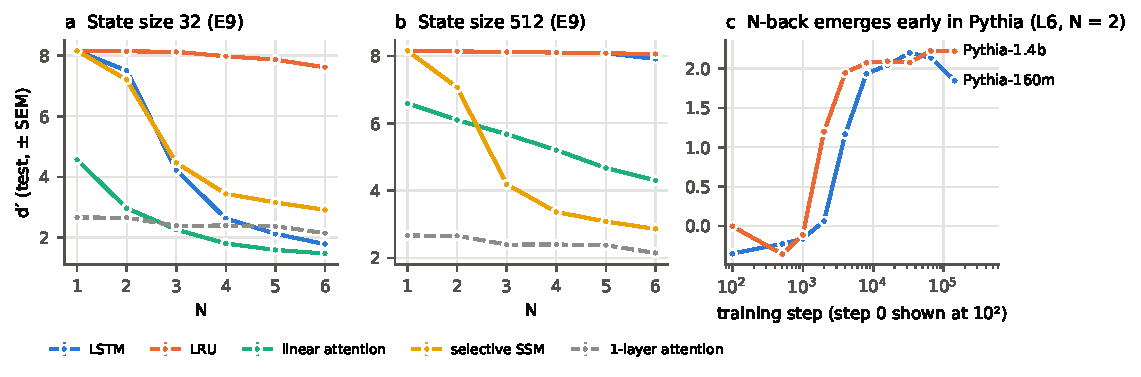
\includegraphics[width=\textwidth]{fig6_architectures_development.pdf}
  \caption{\textbf{Other architectures and development.} (a, b) Recurrent and linear-attention baselines at state sizes 32 and 512, with the one-layer attention model (dashed) for reference; LSTM-512 overlaps LRU-512. (c) N-back \dprime{} over Pythia training (N = 2).}
  \label{fig:arch}
\end{figure}

\section{Additional results}
\label{app:results}

\begin{table}[h]
  \centering\small
  \caption{\dprime{} by model and N (line-by-line format, correct earlier answers shown), and false-alarm rates on N$\pm$1 lures versus other non-matches at N = 2.}
  \label{tab:l2}
  \begin{tabular}{lrrrrrrr}
\toprule
Model & $N{=}1$ & 2 & 3 & 4 & 5 & 6 & lure FA, $N{=}2$ \\
\midrule
Pythia-70m & 1.25 & 1.52 & 1.40 & 0.03 & 0.45 & -0.06 & 0.83 / 0.12 \\
Pythia-160m & 2.10 & 1.85 & 1.92 & 0.96 & 0.79 & 0.10 & 0.79 / 0.02 \\
Pythia-410m & 2.37 & 1.76 & 1.25 & 0.53 & 0.56 & 0.44 & 0.76 / 0.04 \\
Pythia-1b & 2.57 & 2.06 & 1.46 & 0.64 & 0.73 & 0.54 & 0.83 / 0.04 \\
Pythia-1.4b & 3.03 & 2.21 & 1.36 & 0.99 & 0.74 & 0.80 & 0.73 / 0.02 \\
Pythia-2.8b & 2.71 & 2.10 & 1.42 & 0.94 & 0.87 & 0.63 & 0.82 / 0.03 \\
Pythia-6.9b & 3.19 & 1.93 & 1.26 & 1.07 & 1.08 & 1.00 & 0.64 / 0.03 \\
GPT-2 & 2.15 & 2.08 & 1.28 & 0.87 & 0.73 & -0.02 & 0.96 / 0.08 \\
GPT-2 medium & 2.27 & 1.92 & 1.35 & 0.95 & 0.89 & 0.50 & 0.92 / 0.06 \\
GPT-2 large & 2.36 & 2.24 & 1.43 & 0.91 & 0.67 & 0.21 & 0.95 / 0.04 \\
GPT-2 xl & 2.34 & 1.48 & 0.93 & -0.01 & 0.16 & 0.15 & 0.70 / 0.06 \\
Qwen2.5-0.5B & 2.58 & 1.64 & 1.04 & 0.64 & 0.52 & 0.52 & 0.81 / 0.06 \\
Qwen2.5-1.5B & 2.86 & 2.18 & 1.75 & 1.18 & 1.26 & 0.76 & 0.65 / 0.01 \\
Qwen2.5-7B & 3.17 & 1.53 & 1.44 & 0.88 & 0.61 & 0.79 & 0.64 / 0.06 \\
Qwen2.5-14B & 4.28 & 2.42 & 1.60 & 1.29 & 1.41 & 1.15 & 0.63 / 0.01 \\
\bottomrule
\end{tabular}

\end{table}

\begin{table}[h]
  \centering\small
  \caption{Change in \dprime{} under each intervention; bold entries have 95\% bootstrap intervals excluding zero. $^\dagger$ degenerate baseline (excluded from summaries).}
  \label{tab:b1}
  \begin{tabular}{lrrrrrrr}
\toprule
Model & $N$ & base $d'$ & sharpen & ablate top & ablate rand. & suppress & supp. rand. \\
\midrule
Pythia-70m & 2 & 1.52 & \textbf{-0.11} & \textbf{-1.71} & \textbf{-1.08} & \textbf{+0.38} & \textbf{-0.30} \\
 & 3 & 1.40 & \textbf{+0.22} & \textbf{-1.49} & \textbf{-1.28} & \textbf{+0.05} & \textbf{-0.21} \\
 & 4 & 0.03$^\dagger$ & \textbf{+0.97} & \textbf{-0.17} & +0.04 & \textbf{+0.82} & \textbf{+0.31} \\
\addlinespace[2pt]
Pythia-160m & 2 & 1.85 & \textbf{+0.14} & \textbf{-1.62} & +0.01 & \textbf{+1.25} & \textbf{+0.29} \\
 & 3 & 1.92 & \textbf{-0.17} & \textbf{-1.90} & \textbf{-0.13} & \textbf{+0.30} & +0.03 \\
 & 4 & 0.96 & \textbf{+0.30} & \textbf{-1.09} & \textbf{-0.20} & \textbf{-0.22} & +0.01 \\
\addlinespace[2pt]
Pythia-410m & 2 & 1.76 & \textbf{+0.17} & \textbf{-1.36} & \textbf{-0.03} & \textbf{+0.61} & -0.01 \\
 & 3 & 1.25 & \textbf{-0.08} & \textbf{-1.18} & \textbf{+0.13} & \textbf{+0.60} & \textbf{-0.04} \\
 & 4 & 0.53 & \textbf{+0.13} & \textbf{-0.39} & \textbf{+0.08} & \textbf{+0.70} & \textbf{+0.05} \\
\addlinespace[2pt]
Pythia-1b & 2 & 2.06 & \textbf{-0.04} & \textbf{-1.81} & \textbf{+0.13} & \textbf{+0.59} & \textbf{-0.05} \\
 & 3 & 1.46 & \textbf{+0.11} & \textbf{-1.70} & \textbf{+0.34} & \textbf{+0.26} & \textbf{-0.12} \\
 & 4 & 0.64 & \textbf{+0.09} & \textbf{-0.83} & \textbf{+0.29} & \textbf{+0.39} & \textbf{-0.09} \\
\addlinespace[2pt]
Pythia-1.4b & 2 & 2.21 & \textbf{+0.08} & \textbf{-1.61} & \textbf{-0.06} & \textbf{+0.95} & \textbf{-0.05} \\
 & 3 & 1.36 & \textbf{+0.05} & \textbf{-0.93} & \textbf{+0.05} & \textbf{+0.46} & \textbf{+0.05} \\
 & 4 & 0.99 & \textbf{+0.05} & \textbf{-0.66} & +0.02 & \textbf{+0.44} & \textbf{-0.07} \\
\addlinespace[2pt]
Pythia-2.8b & 2 & 2.10 & \textbf{-0.05} & \textbf{-1.59} & \textbf{-0.12} & \textbf{+0.25} & \textbf{-0.03} \\
 & 3 & 1.42 & \textbf{+0.12} & \textbf{-1.01} & \textbf{-0.03} & \textbf{+0.34} & -0.01 \\
 & 4 & 0.94 & \textbf{+0.12} & \textbf{-0.70} & \textbf{+0.02} & \textbf{+0.41} & \textbf{+0.05} \\
\addlinespace[2pt]
Pythia-6.9b & 2 & 1.93 & \textbf{+0.03} & \textbf{-1.02} & \textbf{-0.08} & \textbf{+0.94} & \textbf{-0.08} \\
 & 3 & 1.26 & \textbf{+0.10} & \textbf{-0.34} & \textbf{+0.26} & \textbf{+1.47} & \textbf{+0.13} \\
 & 4 & 1.07 & \textbf{+0.07} & \textbf{-0.55} & +0.03 & \textbf{+1.13} & \textbf{+0.09} \\
\addlinespace[2pt]
GPT-2 & 2 & 2.08 & \textbf{-0.30} & \textbf{-2.20} & \textbf{-0.09} & \textbf{+0.05} & \textbf{-0.22} \\
 & 3 & 1.28 & -0.00 & \textbf{-1.12} & \textbf{-0.09} & \textbf{+0.71} & \textbf{-0.07} \\
 & 4 & 0.87 & \textbf{-0.02} & \textbf{-0.86} & \textbf{+0.07} & \textbf{+0.32} & \textbf{-0.12} \\
\addlinespace[2pt]
GPT-2 medium & 2 & 1.92 & +0.02 & \textbf{-1.38} & \textbf{+0.14} & \textbf{+1.05} & +0.00 \\
 & 3 & 1.35 & \textbf{-0.06} & \textbf{-1.43} & \textbf{-0.10} & \textbf{+0.86} & \textbf{-0.08} \\
 & 4 & 0.95 & \textbf{-0.07} & \textbf{-0.98} & \textbf{-0.18} & \textbf{+0.34} & \textbf{-0.12} \\
\addlinespace[2pt]
GPT-2 large & 2 & 2.24 & \textbf{-0.17} & \textbf{-1.16} & \textbf{-0.09} & \textbf{+0.68} & \textbf{+0.06} \\
 & 3 & 1.43 & \textbf{+0.15} & \textbf{-0.89} & \textbf{+0.02} & \textbf{+0.77} & \textbf{-0.03} \\
 & 4 & 0.91 & \textbf{+0.06} & \textbf{-0.50} & \textbf{-0.05} & \textbf{+0.55} & \textbf{-0.03} \\
\addlinespace[2pt]
GPT-2 xl & 2 & 1.46 & \textbf{+0.12} & \textbf{-1.24} & \textbf{-0.06} & \textbf{+0.52} & \textbf{+0.15} \\
 & 3 & 0.94 & \textbf{+0.12} & \textbf{-0.88} & +0.01 & \textbf{+0.81} & \textbf{-0.05} \\
 & 4 & -0.02$^\dagger$ & \textbf{+0.55} & \textbf{-0.16} & \textbf{+0.53} & \textbf{+0.91} & \textbf{+0.48} \\
\addlinespace[2pt]
Qwen2.5-0.5B & 2 & 1.64 & \textbf{-0.03} & \textbf{-0.87} & \textbf{+0.06} & \textbf{+0.49} & \textbf{+0.15} \\
 & 3 & 1.04 & \textbf{+0.05} & \textbf{-0.65} & \textbf{-0.11} & \textbf{+0.67} & \textbf{-0.07} \\
 & 4 & 0.64 & -0.01 & \textbf{-0.38} & +0.02 & \textbf{+0.60} & \textbf{-0.09} \\
\addlinespace[2pt]
Qwen2.5-1.5B & 2 & 2.18 & \textbf{+0.10} & \textbf{-0.76} & \textbf{+0.06} & \textbf{+0.89} & \textbf{-0.11} \\
 & 3 & 1.75 & +0.01 & \textbf{-0.93} & \textbf{-0.05} & \textbf{+1.15} & +0.01 \\
 & 4 & 1.18 & \textbf{-0.04} & \textbf{-0.78} & \textbf{-0.11} & \textbf{+0.28} & \textbf{-0.09} \\
\addlinespace[2pt]
Qwen2.5-7B & 2 & 1.53 & +0.01 & \textbf{-0.27} & \textbf{+0.06} & \textbf{+0.41} & \textbf{+0.04} \\
 & 3 & 1.44 & \textbf{-0.11} & \textbf{-0.29} & -0.02 & \textbf{+0.99} & \textbf{+0.20} \\
 & 4 & 0.88 & +0.00 & +0.03 & +0.00 & \textbf{+0.63} & \textbf{+0.14} \\
\addlinespace[2pt]
Qwen2.5-14B & 2 & 2.42 & \textbf{+0.05} & \textbf{-0.48} & \textbf{-0.04} & \textbf{+0.46} & \textbf{-0.10} \\
 & 3 & 1.60 & +0.01 & \textbf{-0.17} & +0.01 & \textbf{+1.78} & \textbf{-0.05} \\
 & 4 & 1.29 & \textbf{+0.13} & \textbf{-0.21} & \textbf{+0.07} & \textbf{+0.76} & \textbf{+0.18} \\
\addlinespace[2pt]
\bottomrule
\end{tabular}

\end{table}

\begin{table}[h]
  \centering\small
  \caption{Locating analysis (share of misses with attention off target, on target but lost in later layers, or on target with the heads' output already wrong) and probe results (AUC of the model's own decision and of the probe for matches versus lures, and share of the model's lure false alarms the probe classifies as lures) per model.}
  \label{tab:l7l8}
  \setlength{\tabcolsep}{4.5pt}
  \begin{tabular}{lrrrrrrr}
\toprule
& & \multicolumn{3}{c}{L7: share of misses} & \multicolumn{3}{c}{L8: match vs.\ lure} \\
\cmidrule(lr){3-5}\cmidrule(lr){6-8}
Model & $N$ & elsewhere & lost later & head wrong & model AUC & probe AUC & FA called lure \\
\midrule
Pythia-70m & 2 & 0.08 & 0.49 & 0.43 & 0.58 & 0.97 & 0.75 \\
 & 3 & 0.01 & 0.42 & 0.57 & 0.57 & 0.91 & 0.61 \\
Pythia-160m & 2 & 0.26 & 0.34 & 0.40 & 0.63 & 0.98 & 0.82 \\
 & 3 & 0.03 & 0.59 & 0.38 & 0.58 & 0.99 & 0.85 \\
Pythia-410m & 2 & 0.11 & 0.36 & 0.53 & 0.66 & 1.00 & 0.95 \\
 & 3 & 0.06 & 0.40 & 0.54 & 0.58 & 0.98 & 0.84 \\
Pythia-1b & 2 & 0.11 & 0.32 & 0.57 & 0.68 & 1.00 & 0.95 \\
 & 3 & 0.06 & 0.30 & 0.64 & 0.60 & 0.98 & 0.87 \\
Pythia-1.4b & 2 & 0.12 & 0.72 & 0.16 & 0.76 & 1.00 & 0.99 \\
 & 3 & 0.06 & 0.38 & 0.56 & 0.62 & 0.99 & 0.92 \\
Pythia-2.8b & 2 & 0.04 & 0.36 & 0.60 & 0.71 & 1.00 & 1.00 \\
 & 3 & 0.04 & 0.38 & 0.58 & 0.60 & 1.00 & 0.96 \\
Pythia-6.9b & 2 & 0.19 & 0.55 & 0.26 & 0.74 & 1.00 & 1.00 \\
 & 3 & 0.08 & 0.38 & 0.54 & 0.60 & 1.00 & 0.98 \\
GPT-2 & 2 & 0.16 & 0.65 & 0.19 & 0.49 & 0.97 & 0.84 \\
 & 3 & 0.12 & 0.38 & 0.50 & 0.48 & 0.84 & 0.53 \\
GPT-2 medium & 2 & 0.18 & 0.53 & 0.29 & 0.48 & 0.99 & 0.87 \\
 & 3 & 0.07 & 0.39 & 0.54 & 0.47 & 0.86 & 0.57 \\
GPT-2 large & 2 & 0.72 & 0.15 & 0.13 & 0.56 & 0.99 & 0.92 \\
 & 3 & 0.54 & 0.20 & 0.26 & 0.50 & 0.88 & 0.59 \\
GPT-2 xl & 2 & 0.15 & 0.42 & 0.43 & 0.60 & 1.00 & 0.92 \\
 & 3 & 0.10 & 0.28 & 0.62 & 0.49 & 0.89 & 0.69 \\
Qwen2.5-0.5B & 2 & 0.16 & 0.50 & 0.34 & 0.62 & 1.00 & 1.00 \\
 & 3 & 0.09 & 0.23 & 0.67 & 0.53 & 0.99 & 0.91 \\
Qwen2.5-1.5B & 2 & 0.17 & 0.42 & 0.41 & 0.78 & 1.00 & 1.00 \\
 & 3 & 0.04 & 0.39 & 0.57 & 0.67 & 0.99 & 0.86 \\
Qwen2.5-7B & 2 & 0.14 & 0.43 & 0.43 & 0.63 & 1.00 & 0.98 \\
 & 3 & 0.45 & 0.19 & 0.36 & 0.60 & 0.98 & 0.88 \\
Qwen2.5-14B & 2 & 0.68 & 0.17 & 0.14 & 0.81 & 1.00 & 1.00 \\
 & 3 & 0.51 & 0.13 & 0.36 & 0.64 & 1.00 & 0.95 \\
\bottomrule
\end{tabular}

\end{table}

\textbf{Post-hoc attention edits in the minimal model.} On the 720 one-layer models (the 300 main models and 420 variants; Appendix~\ref{app:methods}), a fixed split of attention between $i$ and $i-N$ gives \dprime{}~$\approx0$ at every N; keeping only the model's own weight on $i$ and $i-N$ lowers \dprime{} from 2.70 to 0.63 at N = 1 and from 2.18 to 1.32 at N = 6, with false alarms rising from 0.03 to 0.67 at N = 1. Removing either the content or the position term of the scores gives \dprime{}~$\approx0$ (content removed: $|d'|\le0.04$; position removed: $-0.28$ to $-0.03$, because content alone cannot tell distance N from any other repeat). Sharpening the trained attention lowers \dprime{} at N = 1--5 and gains at most $+0.06$ at N = 6.


\end{document}
